\chapter{Evaluation}
\label{chap:eval}

\section{Methodology}

\subsection{Test Environment}

The evaluation was conducted on real distributed infrastructure provided by Selectel, ensuring representative network conditions and resource constraints similar to production deployments. The test infrastructure consisted of:

\begin{itemize}
\item \textbf{Infrastructure Provider}: Selectel cloud platform
\item \textbf{Architecture}: 3 nodes (1 control plane, 2 agents)
\item \textbf{Node Configuration}: Each node configured with 2 vCPU and 4 GB RAM
\item \textbf{Platform}: AMD64 architecture
\item \textbf{Control Plane}: Deployed and exposed on port 8080
\item \textbf{Agent Nodes}: 2 agents deployed on separate nodes, each configured with resource reservations for CPU and memory
\item \textbf{Container Runtime}: Docker Engine for container lifecycle management
\item \textbf{Database}: PostgreSQL 16 hosting the application schema with all migrations applied
\end{itemize}

\subsection{Test Scenarios}

Four comprehensive test scenarios were developed to validate system functionality and measure key performance metrics. To establish strong statistical validity, scenarios were executed with multiple trials: BasicWorkloadAcquisition (200 trials), MultipleWorkloads (100 trials), Rescheduling (100 trials), and ConcurrentWorkloads (10 trials).

\begin{enumerate}
\item \textbf{BasicWorkloadAcquisition}: Single workload creation and scheduling to verify basic orchestration functionality
\item \textbf{MultipleWorkloads}: Two workloads created simultaneously to test concurrent scheduling
\item \textbf{Rescheduling}: Agent failure simulation to measure recovery time and automatic rescheduling
\item \textbf{ConcurrentWorkloads}: Multiple workloads scheduled on a single node to test resource management
\end{enumerate}

All tests followed a black-box approach, interacting exclusively through the control plane API and verifying expected state transitions in the database and container runtime.

\subsection{Metrics Definition}

Two primary metrics were measured to evaluate system performance:

\begin{itemize}
\item \textbf{Service Level Objective (SLO)}: Time from workload creation request to the control plane marking the workload status as \texttt{active}. This metric measures how quickly the system can schedule and initialize new workloads.

\item \textbf{Recovery Time Objective (RTO)}: Time from node failure (process termination) to the control plane marking the workload status as \texttt{active} on a different node. This metric measures the system's ability to recover from node failures.
\end{itemize}

The \texttt{active} status is used as the completion criterion because it indicates that the control plane has confirmed successful workload initialization, representing the end-to-end scheduling latency including lease acquisition, container creation, and status reporting.

\section{Test Results}

\subsection{Service Level Objective (SLO)}

Table~\ref{tab:slo-results} presents the SLO measurements across different workload scenarios, including percentile values and 95\% confidence intervals.

\begin{table}[h]
\centering
\resizebox{\textwidth}{!}{\csvautotabular{figs/slo_results_extended.csv}}
\caption{Service Level Objective (SLO) measurements with confidence intervals and percentiles}
\label{tab:slo-results}
\end{table}

The single workload scenario demonstrates that the system can schedule individual workloads with an average time of 15.6 seconds (95\% CI: [15.0s, 16.2s]). The P95 latency of 24.6 seconds indicates that 95\% of workloads are scheduled within this bound, providing a reliable upper estimate for capacity planning.

When scheduling two workloads simultaneously, the average SLO increases to 17.9 seconds (95\% CI: [17.0s, 18.9s]). The P95 of 21.4 seconds shows that the typical concurrent scheduling overhead is modest, with a P99 of 22.7 seconds indicating that nearly all concurrent scheduling operations complete within this bound.

A Mann-Whitney U test confirms that the difference between single and concurrent workload SLO distributions is statistically significant (U = 7478.5, p = 0.0006, p < 0.05), indicating that concurrent scheduling introduces a measurable but bounded performance overhead.

Figure~\ref{fig:box-plots} visualizes the distribution of SLO measurements across scenarios, highlighting the concentration of values below 25 seconds and the presence of outliers in the concurrent scenario.

\begin{figure}[h]
\centering
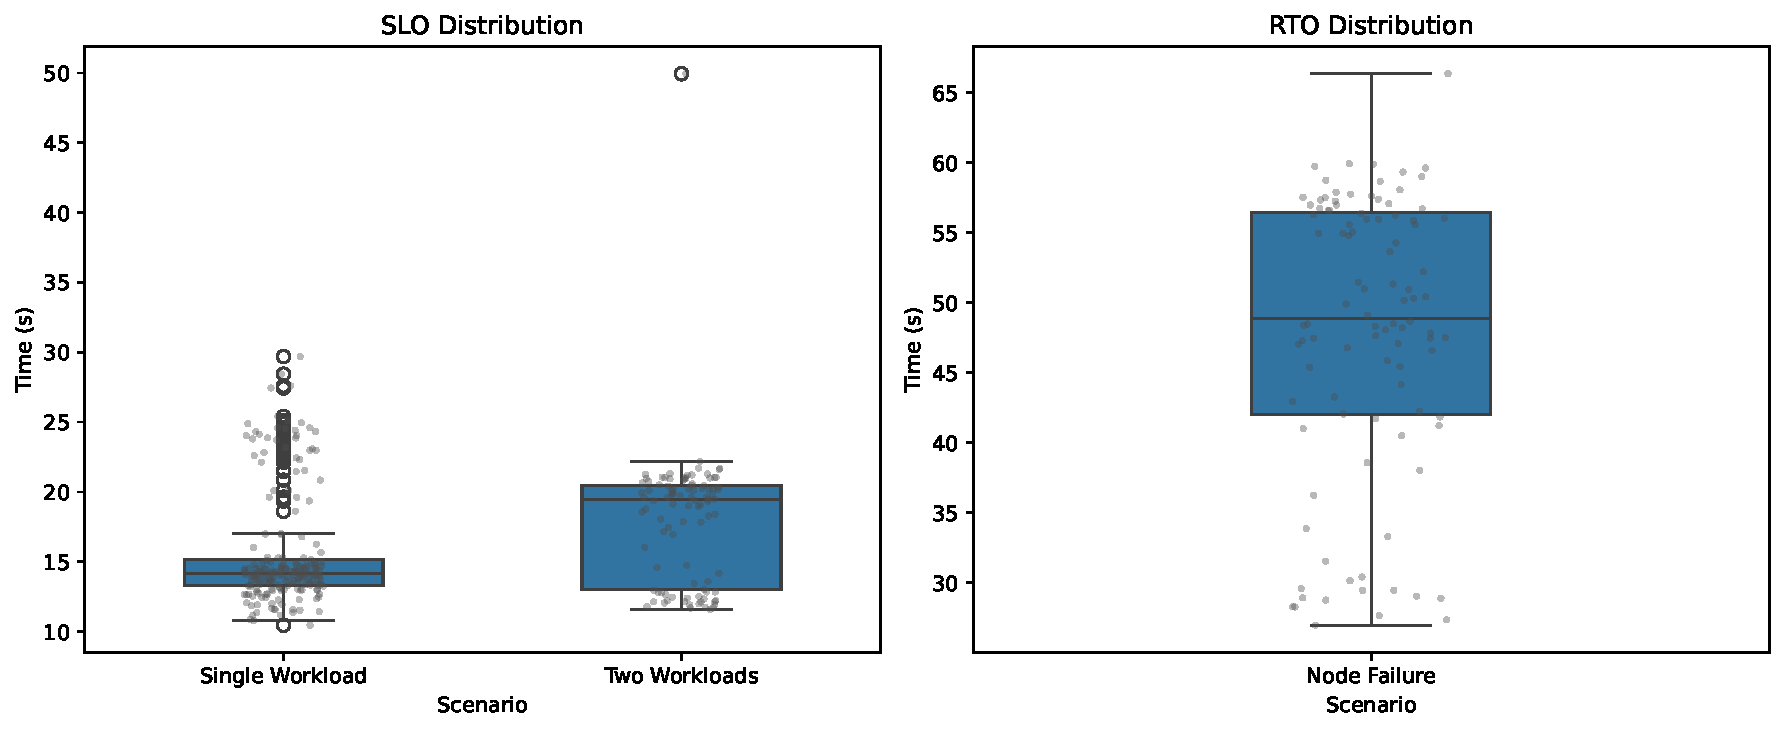
\includegraphics[width=0.9\textwidth]{figs/box_plots.pdf}
\caption{SLO and RTO distribution comparison. Left: SLO for single and concurrent workload scenarios. Right: RTO distribution for node failure recovery. Individual data points are shown as scatter overlay.}
\label{fig:box-plots}
\end{figure}

\subsection{Recovery Time Objective (RTO)}

Table~\ref{tab:rto-results} presents the RTO measurements from node failure scenarios.

\begin{table}[h]
\centering
\resizebox{\textwidth}{!}{\csvautotabular{figs/rto_results_extended.csv}}
\caption{Recovery Time Objective (RTO) measurements with confidence intervals and percentiles}
\label{tab:rto-results}
\end{table}

The RTO measurements demonstrate that the system can recover from node failures with an average time of 47.8 seconds (95\% CI: [45.8s, 49.8s]). The narrow confidence interval ($\pm$2.0 seconds) indicates highly predictable recovery behavior. The P95 of 59.3 seconds provides a reliable upper bound: 95\% of node failures result in workload recovery within one minute.

The RTO is composed of three phases: (1) lease expiration detection (30 seconds), (2) backup agent polling and lease acquisition (2--20 seconds), and (3) container creation and status reporting (approximately 10--15 seconds). The standard deviation of 10.2 seconds indicates moderate variance in recovery times, primarily driven by differences in container startup times and polling alignment.

All 100 trials resulted in successful workload recovery, demonstrating that the lease-based failure detection mechanism operates reliably.

Figure~\ref{fig:cdf} presents the cumulative distribution function for all measured metrics, showing that SLO values converge rapidly while RTO exhibits a more gradual slope due to the fixed 30-second lease timeout component.

\begin{figure}[h]
\centering
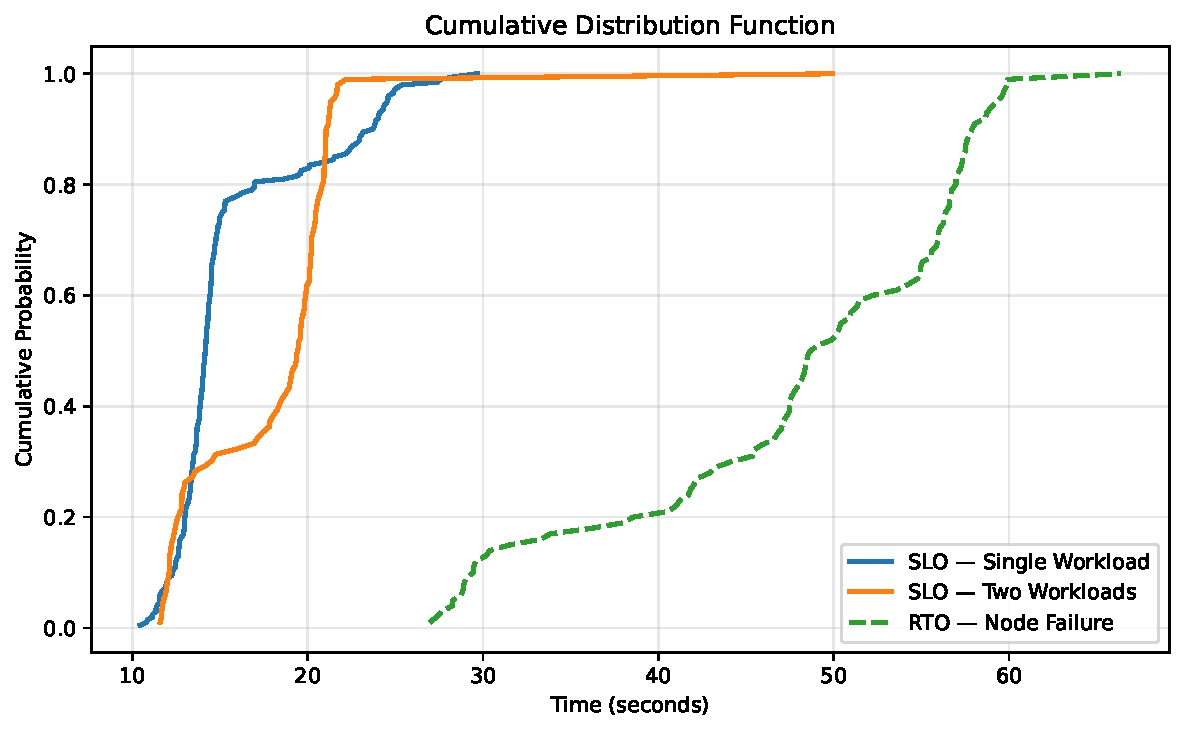
\includegraphics[width=0.8\textwidth]{figs/cdf_plot.pdf}
\caption{Cumulative Distribution Function (CDF) of SLO and RTO measurements. The CDF shows the probability that a measurement falls at or below a given time value.}
\label{fig:cdf}
\end{figure}

\subsection{Functional Validation}

Beyond quantitative metrics, the tests validated core functional requirements:

\begin{itemize}
\item \textbf{Distributed Operation}: Multiple agents successfully coordinated workload assignment without conflicts. The pull-based model with lease exclusivity prevented duplicate workload acquisitions across agents.

\item \textbf{Automatic Rescheduling}: All 100 trials of the rescheduling scenario resulted in successful workload recovery on a different node without manual intervention. The lease expiration mechanism correctly detected node failures and triggered re-acquisition by backup agents.

\item \textbf{Concurrent Workload Handling}: The system successfully handled multiple simultaneous workload creations without resource exhaustion or race conditions. Database transaction isolation ensured correct serialization of concurrent lease acquisition requests.

\item \textbf{Lease Exclusivity}: Each workload was acquired by exactly one agent, with no double-acquisition or lease conflicts observed across 400 total workload placements across all test scenarios.
\end{itemize}

\section{Discussion}

\subsection{Performance Analysis}

The test results demonstrate that the pull-based orchestration model achieves predictable scheduling performance with acceptable latency for short-lived workloads. The average SLO of 15.6 seconds (95\% CI: [15.0s, 16.2s]) for single workloads and 17.9 seconds (95\% CI: [17.0s, 18.9s]) for concurrent workloads is suitable for batch processing, CI/CD pipelines, and other use cases where workload initialization time is not critical compared to total execution time.

The RTO measurements confirm that the lease-based failure detection mechanism provides reliable fault tolerance with a tight confidence interval (95\% CI: [45.8s, 49.8s]). While the 30-second lease timeout introduces a lower bound on failure detection, this trade-off simplifies the architecture by eliminating complex heartbeat protocols and consensus algorithms.

The standard deviation values (4.1 seconds for single SLO, 10.2 seconds for RTO) indicate low to moderate variance. The deterministic nature of the lease expiration mechanism ensures consistent failure detection performance, contributing to the overall predictability of the system.

\subsection{Resource Efficiency}

The control plane was configured with 0.5 vCPU and 1 GB RAM resource limits, representing a minimal footprint compared to existing orchestration platforms. This configuration successfully handled the tested workload (up to 2 concurrent workloads) without performance degradation or resource exhaustion.

Table~\ref{tab:resource-comparison} compares the control plane resource requirements of the proposed system with Kubernetes and HashiCorp Nomad.

\begin{table}[h]
\centering
\begin{tabular}{lcc}
\toprule
Platform & Control Plane CPU & Control Plane Memory \\
\midrule
Kubernetes & 15 vCPU & 22.5 GB \\
Nomad & 3 vCPU & 1.5--2.25 GB \\
Proposed System & 0.5 vCPU & 1 GB \\
\bottomrule
\end{tabular}
\caption{Control plane resource requirements for high-availability deployments. Kubernetes data from \cite{k8s_docs}, Nomad data from \cite{nomad_docs}.}
\label{tab:resource-comparison}
\end{table}

The proposed system achieves a 97\% reduction in CPU overhead and 96\% reduction in memory overhead compared to Kubernetes. Relative to Nomad, the proposed system achieves 83\% lower CPU overhead and 33--56\% lower memory overhead. This efficiency stems from the pull-based architecture, which eliminates complex scheduling algorithms and cluster state management.

\subsection{Design Trade-offs}

The evaluation reveals fundamental trade-offs inherent in the pull-based orchestration model:

\textbf{Simplicity vs. Feature Richness}: The minimalist design yields substantial resource efficiency gains and operational simplicity, but sacrifices advanced features such as sophisticated scheduling algorithms (bin-packing, affinity/anti-affinity), rolling updates, and comprehensive observability. For organizations with simple orchestration requirements, this trade-off is favorable; for complex enterprise deployments, the limitations may be prohibitive.

\textbf{Detection Latency vs. Complexity}: The 30-second lease timeout introduces bounded failure detection latency, but eliminates the need for complex heartbeat protocols and consensus-based failure detection. This trade-off is acceptable for use cases where rapid failure detection is not critical, but may be insufficient for mission-critical applications requiring sub-second recovery times.

\textbf{Scheduling Optimality vs. Scalability}: The first-come-first-served scheduling algorithm may yield suboptimal workload placement compared to global optimization algorithms, but enables linear scalability without scheduling bottlenecks. As the number of agents increases, the pull-based model avoids the scheduler bottleneck that limits push-based systems.

\subsection{Threats to Validity}

Several limitations affect the generalizability of the evaluation findings:

\textbf{Scale Limitations}: The evaluation tested up to 2 concurrent workloads across 2 agents with 100--200 trials per scenario. While this provides strong statistical significance for the tested scale (confirmed by narrow 95\% confidence intervals), large-scale deployments with hundreds of workloads and dozens of agents may exhibit different performance characteristics. Database query performance and connection pool exhaustion become concerns at higher scale.

\textbf{Workload Simplicity}: Test workloads used minimal images (busybox) with simple command execution. Real-world applications with complex initialization logic, dependency resolution, and health check endpoints may exhibit longer startup times and higher resource consumption.

\textbf{Network Homogeneity}: All nodes were deployed in the same Selectel cloud region with low-latency networking. Geographically distributed deployments with higher network latency may exhibit different performance characteristics, particularly for RTO measurements.

\textbf{Test Duration}: Each trial represents a single workflow execution. Long-running tests (hours or days) would be required to detect memory leaks, resource exhaustion, and other emergent behaviors that may not be apparent in short-duration tests.

\section{Conclusion}

This chapter presented empirical evaluation of the pull-based orchestration system, demonstrating predictable scheduling performance (SLO of 15.6 seconds average, 95\% CI: [15.0s, 16.2s]) and reliable fault tolerance (RTO of 47.8 seconds average, 95\% CI: [45.8s, 49.8s]) on real distributed infrastructure. Statistical analysis confirmed that concurrent scheduling introduces a measurable but bounded overhead (Mann-Whitney U test, p = 0.0006). Functional testing validated distributed operation, automatic rescheduling, and concurrent workload handling across 400 total workload placements.

The evaluation confirms that the pull-based architecture achieves substantial resource efficiency gains (97\% CPU reduction, 96\% memory reduction compared to Kubernetes) while maintaining acceptable performance for short-lived workloads. The minimalist design successfully trades feature richness for operational simplicity, making the system suitable for resource-constrained environments and use cases where Kubernetes operational complexity is disproportionate to requirements.

The test results provide evidence that pull-based orchestration is a viable approach for small-scale deployments, offering a compelling alternative for organizations seeking simplicity over feature completeness. Future work should address scalability testing with larger workload counts, long-running stability tests, and performance characterization under network latency and partition scenarios.
